\documentclass[13pt,a4paper]{report}
\usepackage[T1]{fontenc}
\usepackage[utf8]{inputenc}
\usepackage{times}
\usepackage[a4paper,left=2.5cm,right=1.5cm,top=2cm,bottom=2.5cm]{geometry}
\usepackage{setspace}
\usepackage{graphicx}
\usepackage{longtable}
\usepackage{booktabs}
\usepackage{array}
\usepackage{hyperref}
\usepackage{url}
\onehalfspacing

\begin{document}

% Title page (counted as i, hidden number)
\pagenumbering{roman}
\thispagestyle{empty}
\begin{center}
{\large Vietnam National University -- Ho Chi Minh City \\ International University}\\[1.0cm]
{\large Advanced Database System (IT502IU)}\\[1.4cm]
{\LARGE \textbf{Final Report}}\\[0.4cm]
{\Large \textbf{HCMIU Map with Multiple Contributors and Live Updates}}\\[0.8cm]
Project Topic ID \& Name: Individual DBMS Application Project\\[1.2cm]
Student: Huynh Tran Khanh\\
Student ID: MITIU25210\\[0.6cm]
Instructor: Nguyen Thi Thuy Loan\\[2.0cm]
\vfill
\today
\end{center}
\clearpage

\setcounter{page}{2}
\tableofcontents
\clearpage

\chapter*{Abstract}
\addcontentsline{toc}{chapter}{Abstract}
This report presents an ArangoDB-backed collaborative campus map system for Ho Chi Minh City International University. The project integrates two major capabilities: (1) algorithmic indoor navigation (single-source shortest path and multi-stop route planning) and (2) a graph-oriented social knowledge layer where rooms, users, posts, comments, and trial artifacts are linked as first-class entities. The implementation combines a Vite/TypeScript frontend and a Node.js/Express backend, with ArangoDB as the core multi-model database and WebSockets for real-time updates. 

From a database perspective, the most important contribution is an explicit document-and-edge design in which content nodes are stored in document collections and semantic links are persisted in edge collections, enabling relationship-centric queries (reference discovery, full-text exploration, shortest connection paths between entities, and notification fan-out). The report documents architecture, schema decisions, data generation strategy, representative algebraic and query operations, implementation outcomes, and limitations. The system demonstrates that a multi-model DBMS can reduce impedance mismatch in connected applications compared with separating document storage and graph traversal into different engines.

\chapter{Introduction}
\section{System overview}
The system is a web-based collaborative map platform for university indoor spaces. Users can browse floors, compute shortest paths between points, plan multi-stop routes, and open location-linked discussion threads. Beyond mapping, the platform provides social and governance workflows, including follows, notifications, and a ``court trial'' mechanism to discuss and resolve disputes around shared campus knowledge.

\section{Project objectives}
The project objectives are:
\begin{enumerate}
    \item Build an interactive map experience suitable for wayfinding in complex indoor environments, consistent with wayfinding research emphasizing reduced cognitive load in large facilities \cite{zimmerman2006wayfinding}.
    \item Demonstrate advanced database features using ArangoDB's native multi-model architecture (document + graph + search-like querying) \cite{arangodb_multimodel}.
    \item Provide relationship-first collaborative features such as references, degree-of-separation analysis, and event notifications.
    \item Validate correctness through automated API and end-to-end flows.
\end{enumerate}

\section{Techniques and tools used}
The implementation stack includes:
\begin{itemize}
    \item \textbf{DBMS:} ArangoDB 3.11.
    \item \textbf{Backend:} Node.js + Express + arangojs.
    \item \textbf{Realtime:} WebSocket protocol (RFC 6455) \cite{rfc6455}.
    \item \textbf{Frontend:} Vite + TypeScript + CSS.
    \item \textbf{Testing:} Node native test runner and Puppeteer-based scenarios.
    \item \textbf{Containerization:} Docker and Docker Compose.
\end{itemize}

\section{Scope and limitations}
\textbf{Scope.} The project covers indoor map visualization, route planning, collaborative entities/comments, trial negotiation, notification streams, and graph-oriented research APIs.

\textbf{Limitations.}
\begin{itemize}
    \item No GPS/RTLS integration for live indoor positioning.
    \item Full-text search is substring-based in AQL queries, not a dedicated ranked IR engine.
    \item Routing is graph-based over predefined points, so accuracy depends on map graph quality.
\end{itemize}

\section{Report structure}
Chapter 2 presents timeline and personal contribution. Chapter 3 details methodology, DBMS rationale, data design, and representative operations. Chapter 4 discusses implementation outcomes and challenges. Chapter 5 concludes and proposes future work.

\chapter{Project Timeline \& Contribution}
\section{Timeline of milestones}
\begin{longtable}{p{2.8cm}p{4.6cm}p{7.2cm}}
\toprule
\textbf{Week} & \textbf{Phase} & \textbf{Outcome} \\
\midrule
Week 1 & Design \& orchestration & Defined system architecture, Docker orchestration, and initial ArangoDB collections. \\
Week 2 & Backend API implementation & Implemented authentication, entities, references, follows, notifications, and trial APIs. \\
Week 3 & Frontend integration & Connected collaborative UI pages and map-to-entity linking workflows. \\
Week 4 & Testing \& reporting & Executed API/E2E tests, reviewed proposal alignment, and completed final documentation. \\
\bottomrule
\end{longtable}

\section{Work breakdown by phase}
\begin{itemize}
    \item \textbf{Design:} Determined entity model, edge semantics, and event model.
    \item \textbf{Implementation:} Developed backend services and frontend interaction pages.
    \item \textbf{Experimentation:} Executed scenario tests (map entity lookup, research queries, trial flow).
    \item \textbf{Documentation:} Produced API docs and final report.
\end{itemize}

\section{Contribution statement}
All project stages (design, coding, testing, deployment setup, and report writing) were completed individually by the student.

\chapter{Methodology}
\section{Selected DBMS and justification}
ArangoDB was selected because the application requires both document storage (users, entities, trials, notifications) and graph traversal over explicit references/follows. A dedicated property-graph or document-only DBMS would require additional systems or custom join logic for the opposite paradigm. In contrast, ArangoDB natively supports document and graph workloads with AQL in one engine \cite{arangodb_aql,arangodb_multimodel}. This aligns with graph database principles for highly connected data \cite{angles2008property,robinson2015graph}.

\section{Database design}
\subsection{Conceptual ER-style view}
Main conceptual objects:
\begin{itemize}
    \item \textbf{User}: account identity and password hash metadata.
    \item \textbf{Entity}: generic content node (post, comment, user-profile-entity, map location, trial entity).
    \item \textbf{Trial}: dispute case with participants, judge proposals, votes, and status.
    \item \textbf{Notification}: event delivered to a user.
\end{itemize}

Relations:
\begin{itemize}
    \item \textbf{entity\_references} (edge collection): entity $\rightarrow$ entity semantic references.
    \item \textbf{follows}: user follows entity.
\end{itemize}

\subsection{Relational projection (for 3NF discussion)}
Although deployed in ArangoDB, an equivalent normalized relational view is:
\begin{itemize}
    \item \texttt{Users(user\_id PK, username UNIQUE, client\_salt, server\_salt, verifier\_hash, created\_at)}
    \item \texttt{Entities(entity\_id PK, type, title, body, parent\_entity\_id FK, created\_by FK, created\_at)}
    \item \texttt{EntityReferences(from\_entity\_id FK, to\_entity\_id FK, created\_at, PK(from\_entity\_id,to\_entity\_id))}
    \item \texttt{Follows(user\_id FK, entity\_id FK, created\_at, PK(user\_id,entity\_id))}
    \item \texttt{Notifications(notification\_id PK, user\_id FK, entity\_id FK, type, read, created\_at)}
    \item \texttt{Trials(trial\_id PK, plaintiff\_id FK, defendant\_id FK, status, agreed\_judges\_json, votes\_json, created\_at)}
\end{itemize}
This projection is in 3NF for core scalar attributes, with graph edges represented by associative tables.

\section{Data collection and population}
Data sources are mixed:
\begin{itemize}
    \item \textbf{Static map metadata} extracted from source files containing room and lift names.
    \item \textbf{Synthetic user/activity data} generated through UI/API interactions and automated tests.
\end{itemize}
At backend startup, map entities are pre-provisioned for each floor and construct name, creating stable IDs for collaborative threads.

\section{Database queries and operations}
\subsection{Relational algebra examples}
Let $E$ be entities and $R$ be entity\_references.
\begin{itemize}
    \item \textbf{All comments under parent p:}
    \[
    \sigma_{type='comment' \land parentEntityId=p}(E)
    \]
    \item \textbf{Entities that reference target t:}
    \[
    \pi_{E.*}(\sigma_{R.to=t}(R) \bowtie_{R.from=E.id} E)
    \]
\end{itemize}

\subsection{AQL/SQL-style operational mapping}
Representative operations:
\begin{enumerate}
    \item \textbf{DML insert entity}: create document in \texttt{entities}, then synchronize outgoing edges in \texttt{entity\_references}.
    \item \textbf{Complex graph query}: shortest connection path between two entities using \texttt{ANY SHORTEST\_PATH} traversal in AQL.
    \item \textbf{Search query}: case-insensitive text filter across ID/title/body.
\end{enumerate}

The shortest-path operation corresponds to connected-data use cases where graph traversal is preferable to repeated relational self-joins \cite{robinson2015graph}.

\section{Application architecture}
\begin{itemize}
    \item \textbf{Frontend (Vite):} map pages, collaborative dashboard, and research panels.
    \item \textbf{Backend (Express):} auth, entities, trials, notifications, and activity endpoints.
    \item \textbf{Database (ArangoDB):} durable storage and AQL execution.
    \item \textbf{Realtime channel:} WebSocket broadcasts for entity/trial/notification events.
\end{itemize}

\begin{figure}[h]
\centering
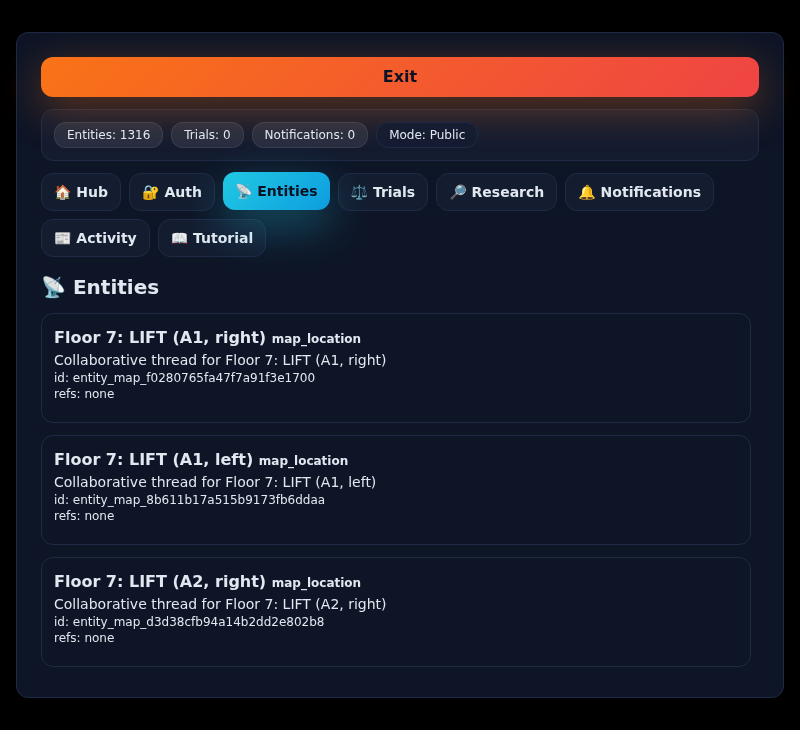
\includegraphics[width=0.9\textwidth]{../docs/screenshots/collaborative-page.png}
\caption{Collaborative page UI snapshot.}
\end{figure}

\begin{figure}[h]
\centering
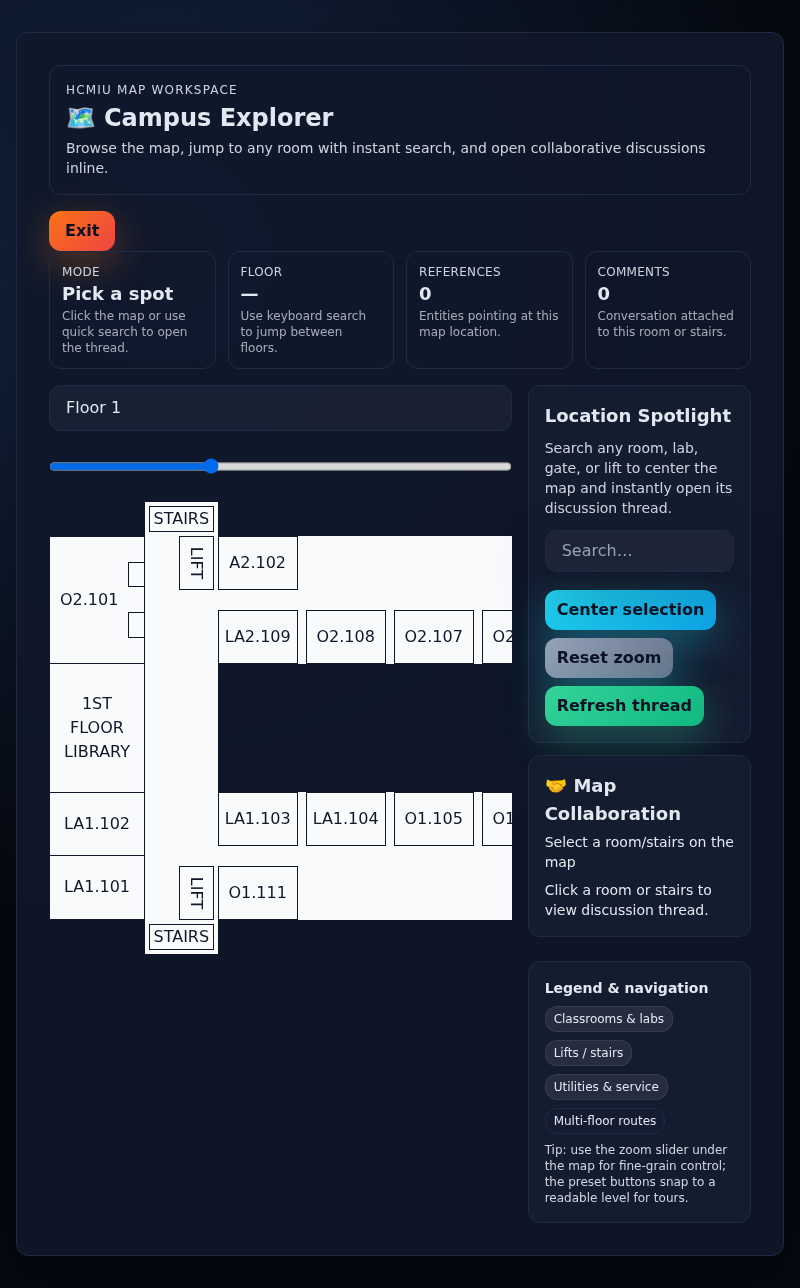
\includegraphics[width=0.9\textwidth]{../docs/screenshots/map-view-page.png}
\caption{Map view page with navigation functionality.}
\end{figure}

\section{User interface design}
The collaborative UI is split into focused pages: Hub, Authentication, Entities, Trials, Research, Notifications, Activity, and Tutorial. This segmentation reduces interaction complexity and supports task-oriented workflows.

\chapter{Discussion \& Implementation}
\section{Implementation process}
The implementation followed an incremental path:
\begin{enumerate}
    \item establish containerized runtime and ArangoDB availability;
    \item implement collection initialization and startup provisioning;
    \item add authentication and entity CRUD;
    \item layer reference edges and research APIs;
    \item implement trial negotiation and voting flows;
    \item integrate frontend workflows and websocket refreshes;
    \item validate with automated scenarios.
\end{enumerate}

\section{Results and analysis}
\textbf{Functional outcomes.}
\begin{itemize}
    \item Map entities are auto-generated and linkable from floor/construct names.
    \item Reference graph operations support inbound reference lookup, text search, and shortest path.
    \item Trial workflow supports proposal/counter-proposal/acceptance before voting.
    \item Notifications and activity feed provide temporal awareness of collaboration.
\end{itemize}

\textbf{Database-level observations.}
\begin{itemize}
    \item Unified AQL over documents and graph edges reduces application-level data stitching.
    \item Edge collection synchronization on entity write ensures referential consistency of outbound references.
    \item Graph traversal query for degree-of-separation is concise compared with equivalent recursive SQL.
\end{itemize}

\textbf{Algorithmic component.}
Shortest-route and multi-stop planning are consistent with classic graph optimization foundations (Dijkstra for shortest path, dynamic programming lineage for TSP variants) \cite{dijkstra1959,bellman1962}.

\section{Challenges and solutions}
\begin{itemize}
    \item \textbf{Challenge:} balancing generic entity schema with feature-specific behavior. \\
    \textbf{Solution:} use typed entities plus dedicated collections for critical workflow state (e.g., trials).
    \item \textbf{Challenge:} real-time consistency between REST writes and UI state. \\
    \textbf{Solution:} broadcast websocket events and re-fetch canonical state on client event receipt.
    \item \textbf{Challenge:} stable linkage between map coordinates and collaborative threads. \\
    \textbf{Solution:} deterministic hashed map-entity ID generation.
\end{itemize}

\chapter{Conclusion \& Future Work}
\section{Summary of key findings}
This project demonstrates that ArangoDB is well-suited for a collaborative campus map where content and relationships are equally important. Document storage supports flexible user-generated content, while graph edges and traversals enable deep relationship queries without external graph infrastructure.

\section{Reflection on objectives}
The primary objectives were achieved: the system provides route planning, multi-user collaboration, graph-oriented research functions, and real-time updates in one deployable stack.

\section{Advanced database implications}
From an advanced DBMS perspective, the work illustrates practical benefits of multi-model design for connected applications, especially where entities evolve rapidly and relationship queries are central.

\section{Future work}
\begin{itemize}
    \item Add ArangoSearch views and ranking for richer retrieval quality.
    \item Introduce fine-grained authorization roles and moderation policies.
    \item Evaluate query performance under larger synthetic workloads.
    \item Integrate optional indoor positioning feeds and accessibility-aware routing.
\end{itemize}

\bibliographystyle{plain}
\bibliography{references}

\end{document}
